\chapter{معماری نمونه مطالعاتی تاکسی‌آنلاین \lr{Uber}}
\section{معماری میکرو‌سرویس دامنه‌گرا}
\label{section:domainmicroservice}
اوبر \LTRfootnote{Uber} دارای بیش از ۲۲۰۰ میکرو‌سرویس است\cite{microservice_uber} و وجود تعداد زیادی میکرو‌سرویس باعث پیدایش پیچیدگی زیادی در نگهداری این سرویس ها و توسعه سرویس‌های جدید می‌شود تا جایی که \lr{Uber} سعی کرد با تغییراتی در معماری میکرو‌سرویس، معماری میکروسرویس دامنه‌گرا\LTRfootnote{Domain-Oriented Microservice Architecture} را ارائه دهد؛ در معماری میکرو‌سرویس دامنه‌گرا سعی شده است تا با حفظ مزیت‌های معماری میکرو‌سرویس، از پیچیدگی کل سیستم کاسته شود.

در معماری میکروسرویس، سرویس‌ها با عملکرد محدود به یک حوزه بر روی یک شبکه مستقر می‌شوند و از طریق رابط های تعریف شده به درخواست‌های که به صورت \lr{Remote Procedure Call} ارسال می‌شوند پاسخ می‌دهند؛ اوبر به دلایل زیر در سال ۲۰۱۲ معماری خود را از \lr{monolithic} به \lr{micro-service} تغییر داد:
\begin{itemize}
\item
ریسک‌های دردسترس‌پذیری\LTRfootnote{Availability} : یک خطا در سیستم \lr{monolithic} می‌توانست منجر به از دست خارج‌شدن کل سیستم \lr{Uber} شود.
\item
استقرار\LTRfootnote{Deployment} های پرخطر و زمان‌بر
\item
تفکیک ضعیف نگرانی‌ها\LTRfootnote{Concerns} : با‌وجود یک پایگاه کد بزرگ تفکیک مرز میان منطق تجاری و مولفه‌ها در یک سیستم با رشد بسیار سریع به خوبی صورت نمی‌پذیرد.
\item
اجرای ناکارآمد : وجود مشکلاتی که به چندین تیم وابستگی دارد، سبب می‌شود تا کارایی در اجرا بسیار پایین باشد.
\end{itemize}

هر چند مهاجرت از سیستم با معماری \lr{monolithic} به \lr{microservice} در زمانی که اندازه شرکت اوبر به صد‌ها مهندس رسیده بود بسیاری از مشکلات را حل کرد، اما زمانی که تعداد میکرو‌سرویس‌ها افزایش یافت شرکت متوجه پیچیدگی روزافزون معماری میکروسرویس شد؛ به عنوان مثال گاهی نیاز است برای یافتن ریشه‌ی یک خطا چندین میکروسرویس از تیم‌های مختلف مورد بررسی قرار گیرند. همچنین وابستگی میان سرویس‌ها گاه سبب می‌شود تا تاخیر پاسخ یک سرویس دیگر قابل قبول نباشد.همان طور که از پیچیدگی شبکه \lr{Uber} در سال ۲۰۱۸ \ref{fig:microserice_network} مشخص است میکروسرویس ها شدیدا به یکدیگر وابسته هستند.
\begin{figure}[h]
\label{fig:microserice_network}
\centering
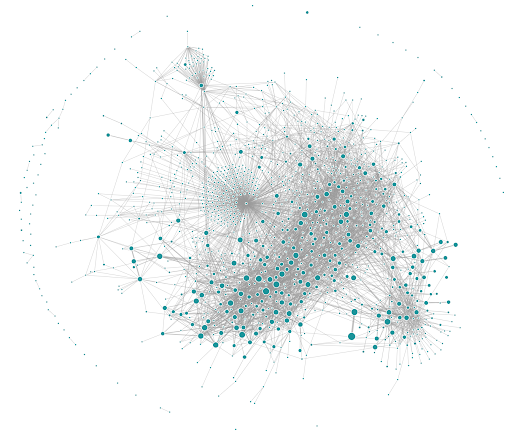
\includegraphics[width=8cm]{uber_service_network.png}
\end{figure}

به جهت پیاده‌سازی یک امکان جدید در \lr{Uber} یک تیم باید با سرویس‌‌های متفاوت متعلق به تیم‌های متفاوت کار کند و این عمل به جلسات زیادی بر روی طراحی و بازبینی کد نیاز دارد. همچنین مزیت معماری میکروسرویس در مورد داشتن خطوط مشخص مالکیت سرویس، هنگامی که تیم ها در سرویس های یکدیگر کد ایجاد می‌کنند، مدل‌های داده یکدیگر را اصلاح می کنند و حتی از طرف دارندگان سرویس نسخه‌های جدید را استقرار\LTRfootnote{deployment} می‌دهند، به خطر می افتد.در نتیجه با افزایش تعداد سرویس‌ها گویا با یک سیستم \lr{Network Monolithic} سر کار داریم که یکی از نتایج آن این است که چندین میکروسرویس به ظاهر مستقل نیاز دارند تا همزمان در سامانه مستقر شوند تا سامانه بدون نقص به عملکرد خود ادامه دهد.

در "معماری سرویس دامنه‌گرا" به طور عمده از روشهای تثبیت‌شده ساختار‌دهی کد مانند طراحی مبتنی بر دامنه \LTRfootnote{Domain-driven Design} \cite{evans2004domain}، معماری تمیز\LTRfootnote{Clean Architecture} \cite{martin2018clean}، معماری سرویس‌گرا\LTRfootnote{Service-Oriented Architecture} \cite{perrey2003service} و الگوهای طراحی شی‌گرا \LTRfootnote{object-oriented design} و رابطه گرا\LTRfootnote{interface-oriented design} استفاده می شود.

اصول اصلی و اصطلاحات مرتبط با معماری سرویس دامنه‌گرا به شرح زیر است:
\begin{itemize}
\item 
با تعریف \lr{Domain} به جای شکل گیری پیرامون یک به یک میکروسرویس‌ها، پیرامون مجموعه‌ای از میکروسرویس‌های مرتبط شکل گرفته است.
\item
معماری \lr{Uber} همچنین مجموعه دامنه هایی را ایجاد می‌کند که لایه نامیده می‌شوند. لایه‌ای که دامنه به آن تعلق دارد مشخص می کند که میکروسرویس‌های موجود در آن دامنه چه وابستگی هایی را دارند.
\item
معماری برای دامنه‌ها رابط هایی مشخص ارائه می‌دهد که به عنوان یک نقطه واحد ورود به مجموعه رفتار می‌کنند و به آن‌ها دروازه\LTRfootnote{gateway} گفته می‌شود.
\item
هر دامنه باید برای دامنه های دیگر ناشناخته باشد ، به عبارت دیگر ، یک دامنه نباید منطق مربوط به دامنه دیگری را داشته باشد که در داخل کد یا مدل داده‌‌ای دامنه دیگر وجود دارد. از آنجا که گاهی تیم ها نیاز دارند تا منطق را در دامنه تیم دیگری قرار دهند، ما یک معماری تکمیلی برای پشتیبانی از نقاط توسعه یافته تعریف شده در دامنه ارائه می دهیم.
\end{itemize}

دامنه‌ها به واسطه گردهمایی سرویس‌هایی که منطق تجاری مشابهی دارند، ایجاد می‌شوند و تعداد سرویس‌های درون یک دامنه متغیری است که دامنه‌ی گسترده‌ای دارد و دامنه ها می توانند شامل یک تا ده ها سرویس باشند؛ به عنوان مثال \lr{Uber Maps} به سه دامنه تقسیم می‌شود که این ۳ دامنه در مجموع ۸۰ میکروسرویس را در بر دارند و ۳ \lr{gateway} بر سر راه آن‌ها تعبیه شده است.

معماری \lr{Uber} برای پاسخ به این سوال که "چه سرویس‌هایی می‌توانند چه سرویس‌های دیگری را فراخوانی کنند" دست به ایجاد لایه‌ها در سطح معماری زده‌است.با وجود لایه‌های مختلف مدیریت وابستگی در مقیاس صورت می‌پذیرد و نگرانی‌های مختلف معماری در لایه‌‌های مختلف از یکدیگر تفکیک می‌شوند.به کمک لایه‌ها با در نظر گرفتن شعاع انفجار شکست\LTRfootnote{failure blast radius}  دامنه‌ها، دامنه‌هایی که در پایین هرم قرار می‌گیرند وابستگی‌‌های بیشتری داشته و مجموعه‌ی بزرگتری از عملکرد‌‌های تجاری را ارائه می‌دهند.شکل \ref{fig:layers} به خوبی ایده‌ی لایه‌بندی را نشان می‌دهد:

\begin{figure}[h]
\centering
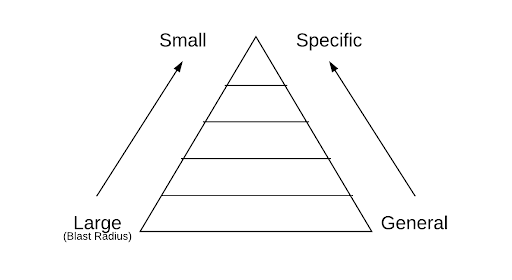
\includegraphics[scale=0.5]{layers.png}
\caption{لایه ها}
\label{fig:layers}
\end{figure}

لایه‌های پایینی عملکرد‌هایی نظیر مدیریت حساب کاربران را پشتیبانی می‌کنند در حالی که در قله هرم به عملکرد‌های جزئی‌تر نظیر تجربه کاربری یک امکان در موبایل پرداخته می‌شود.امکانات ممکن است با پخته‌تر شد تعمیم داده شوند و به لایه‌های پایین تر هرم مهاجرت کنند.

شرکت \lr{Uber} از ۵ لایه‌ی زیر در معماری لایه‌های خود استفاده می‌کند:
\begin{itemize}
\item
لایه زیرساخت\LTRfootnote{Infrastructure Layer} : پاسخ سوالاتی که هر واحد مهندسی می‌تواند از آن استفاده کند نظیر فضای ذخیره‌سازی و شبکه در این لایه داده شده است.
\item
لایه تجاری\LTRfootnote{Business Layer} : عملکرد‌های تجاری که سازمان عبور می‌تواند استفاده کند اما منحصرا مربوط به یک محصول خاص نظیر \lr{Uber Ride} یا \lr{Uber Eat} نیستند در این لایه قرار می‌گیرد.
\item
لایه محصول \LTRfootnote{Product Layer} : عملکرد‌های تجاری که مربوط به یک محصول و خط کسب‌و‌کار است توسط این لایه تامین می‌شود اما این لایه نیاز های مختص به یک پلتفرم خاص را پیاده‌سازی نمی‌کند؛ به عنوان به مثال به نحوه پیاده سازی "درخواست سفر" در اپلیکیشن موبایل کاری ندارد.
\item
لایه نمایش \LTRfootnote{Presentaion layer} : نیاز‌های عملکردی که کاربران در زمان استفاده از یک برنامه و پلتفرم خاص نیاز دارند را برطرف می‌کند.
\item
لایه لبه \LTRfootnote{Edge Layer} : لایه لبه امکانات \lr{Uber} را به دنیای بیرون عرضه می‌کنند و اپلیکیشن‌های موبایل نیز از ویژگی‌های این لایه استفاده می‌کنند.
\end{itemize}

همان‌طور که مشاهده می‌شود هر چه به لایه‌های بالاتر می‌رویم میزان شعاع انفجار شکست کاهش می‌یابد و عملکرد دامنه‌ها خاص‌تر می‌شود.

دروازه‌های تعریف شده در معماری میکروسرویس دامنه‌گرا بجای اینکه به یک میکروسرویس مربوط باشد به مجموعه‌ای از میکروسرویس‌ها که ما از آن‌ها با نام دامنه یاد می‌کنیم مربوط هستند.شکل \ref{fig:gateways} به خوبی ارتباط را نمایش می‌دهد.‍

\begin{figure}[h]
\centering
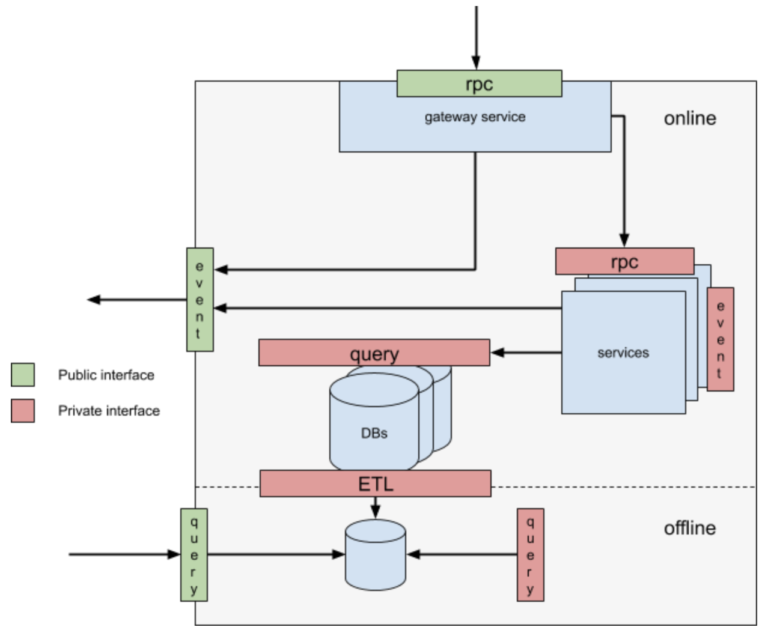
\includegraphics[scale=0.5]{gateways.png}
\caption{دروازه ها}
\label{fig:gateways}
\end{figure}

اگر به معنای طراحی شی گرا به دروازه ها نگاه شود، دروازه‌ها در واقع تعاریف واسط هستند، که به ما امکان می دهد هر کاری را که می خواهیم از نظر "پیاده سازی" در پایگاه کد انجام دهیم.

\section{قابل مشاهده بودن در مقیاس بزرگ}
در هنگام تصور سازمانی به بزرگی \lr{Uber} یکی از نیاز‌های مهم قابلیت مشاهده و مانیتورینگ بسیاری از نیاز‌های کیفی همراه با رشد و گسترش سازمان است. برای حفظ ثبات در معماری میکروسرویس دامنه‌گرا که در بخش \cite{domainmicroservice} به آن اشاره شد تیم مشاهده\LTRfootnote{Obserability team} شرکت \lr{Uber} اقدام به ساخت خط لوله‌هایی به منظور تشخیص، هشدار و کاهش عواقب مشکلات در میکروسرویس‌های ساخته‌شده در تیم‌های مهندسی مختلف کرده‌است؛ به عنوان مثال دو نمونه از این خط لوله‌ها به جهت مراقبت از دیتاسنتر‌ها با نام‌های \lr{uMonitor} و \lr{Neris} ساخته شده اند.\lr{uMonitor} سیستم هشدار مبتنی بر معیار‌ها در \lr{Uber} است که بر اساس پلتفرم \lr{M2} \cite{m3_uber} مراکز داده را بررسی می‌کند، در حالی که \lr{Neris} در درجه اول به دنبال هشدارها در زیرساخت های سطح میزبان است.

\section{مدیریت منابع در \lr{Uber}}
یکی زیرساخت‌های نرم افزاری رایج در بین شرکتهای فناوری کلاستر\LTRfootnote{cluster} ها هستند.کلاستر مجموعه‌ای از منابع با میزبان‌های فیزیکی متفاوت است که با تبدیل به یک منبع مشترک منطقی در جهت تقویت توان محاسباتی و استفاده انعطاف پذیر از سخت افزار مراکز داده فعالیت می‌کند. در \lr{Uber}، مدیریت کلاسترها یک لایه انتزاعی برای کارهای مختلف فراهم می کند\cite{resource_uber}.

با افزایش گستره تجارت \lr{Uber} استفاده کارآمد از منابع کلاستر‌ها بسیار مهم می شود.پشته محاسباتی \lr{Uber} به دلیل وجود کلاستر های اختصاصی برای موارد استفاده دسته‌ای\LTRfootnote{Batch} ، باوضعیت\LTRfootnote{Stateful} و بی‌وضعیت\LTRfootnote{Stateless} به مدیریت ویژه‌ای نیازمند است و همچنین ماهیت دینامیک کسب‌و‌کار \lr{Uber} این مساله را سخت‌تر نیز می‌سازد؛ به عنوان مثال دامنه تقاضا برای سفرها با توجه به تعطیلات و ایام هفته بسیار متغیر است.هر چند \lr{Uber} سعی کرده است تا با فراهم آوردن سخت‌افزار بیش از حد نیاز تا جای ممکن در پاسخ به نیاز مشتریان کاستی نداشته باشد اما گاهی در هنگام اوج بار یک محصول و خط کسب‌و‌کار، درست در زمانی که بخشی از کلاستر‌ها اضافه بار دارند، کلاستر سایر محصولات ممکن است فضای خالی بدون استفاده داشته باشند و این تکیه بر کلاستر‌های اختصاصی نیز به این معنی است که  \lr{Uber} نمی‌تواند منابع محاسبه ای را بین آنها به اشتراک بگذارد.


برای استفاده بهتر از منابع،\lr{Uber} باید این بارهای کاری را در یک سیستم مدیریت بار واحد محاسبه کند. افزایش کارایی‌های حاصل باعث کاهش هزینه فنی هر سفر در زیرساخت های \lr{Uber} می‌شود و باعث افزاش حاشیه سود سفر‌ها در \lr{Uber} و درنهایت به نفع رانندگان و مسافران خواهد شد.

راه حلی که \lr{Uber} برای مدیریت کلاستر ها ارائه کرده است نرم‌افزار مدیریت یکپارچه کلاستر ها به نام \lr{Peloton} است\cite{resource_uber}؛ \lr{Peloton} یک برنامه‌ریز یکپارچه است که برای مدیریت منابع در بارهای متمایز طراحی شده است و مدیریت کلاستر ها در \lr{Uber} را تجمیع می‌کند. \lr{Peloton} با استفاده از یک پلتفرم مشترک، توازن در استفاده از منابع، به اشتراک گذاری گسترده منابع و پیش‌بینی استفاده از منابع برای نیازهای آینده در \lr{Uber} را پشتیبانی می‌کند.

از سایر محصولات مشابه با \lr{Peloton} می‌توان به \lr{Google Borg}\cite{verma2015large} ،\lr{kubernetes}\cite{kubernetes} ، \lr{Hadoop YARN}\cite{hadoop} و \lr{Apache Mesos/Aurora}\cite{aurora}\cite{mesos} اشاره کرد.

\section{منابع ذخیره‌سازی داده در \lr{Uber}}
پیش از سال ۲۰۱۶ شرکت \lr{Uber} از پایگاه داده \lr{Postgres} استفاده می‌کرد \cite{migration_postgres}، اما امروز با استفاده از روشی بدون طرح\LTRfootnote{Schemaless}\cite{schemaless}  با ترکیب تکنولوژی‌هایی نظیر \lr{Riak}\cite{riak} و \lr{cassandra}\cite{cassandra} به همراه \lr{MySql}   داده‌هایی که برای طولانی مدت نیاز به نگهداری دارند، را ذخیره سازی می‌کند.در طول زمان \lr{Postgres} و \lr{Mysql} جای خود را به موتور‌‌های \lr{Nosql} دادند و همچنین به جهت دست‌یابی هر چه بهتر به ویژگی کیفی کارایی در بسیاری از کاربرد ها با افزایش حجم داده‌ها \lr{Riak} جایگاه خود را به \lr{cassandra} می‌دهد.مهندسانی که ابزارهای کاربردی و چند منظوره را برای پذیرش در سراسر \lr{Uber} ایجاد می کنند،از \lr{Cassandra} و \lr{Go} با شدت بیشتری نسبت به تیم های دیگر در \lr{Uber} استفاده می‌کنند که دلیل اصلی آن سرعت است.همچنین \lr{Uber} از \lr{Redis}\cite{redis}  هم برای ذخیره سازی داده در حافظه‌های سریع و هم برای صف بندی استفاده می کند و با استفاده از \cite{Twemproxy}\lr{Twemproxy} مقیاس پذیری لایه حافظه پنهان را بدون از بین بردن نسبت برخورد\LTRfootnote{Hit Ratio} حافظه نهان از طریق الگوریتم هش کردن سازگار فراهم می کند.

برای ذخیره سازی توزیع شده و تجزیه و تحلیل داده های پیچیده ،از انبار داده \lr{Hadoop}\cite{hadoop} به جهت ذخیره بهینه داده ها استفاده می‌شود.

\section{ثبت وقایع در \lr{Uber}}
در \lr{Uber}،از \lr{Apache Kafka}\cite{kafka} به عنوان یک گذرگاه پیام برای اتصال قسمت های مختلف اکوسیستم استفاده می‌شود.\lr{Uber} لاگ\LTRfootnote{Log} مربوط به سیستم و برنامه ها و همچنین داده های رویداد را از برنامه های رانندگان و مسافران را جمع آوری می‌کند و سپس این داده‌‌ها را از طریق کافکا\LTRfootnote{Kafka} در دسترس مصرف کنندگان پایین دست قرار می‌دهد.

داده ها در کافکا توسط خطوط لوله \lr{real-time} و خطوط دسته‌ای\LTRfootnote{batch} تغذیه می‌شوند. داده های خطوط لوله مربوط به فعالیت هایی مانند محاسبه معیارهای تجاری ،رفع باگ\LTRfootnote{Bug} ،هشدار و داشبورد است.شکل \ref{fig:kafka} نمایی از نحوه ارتباط کافکا با سایر اجزای معماری رد \lr{Uber} را نشان می‌دهد.\cite{kafka}

\begin{figure}[h]
\centering
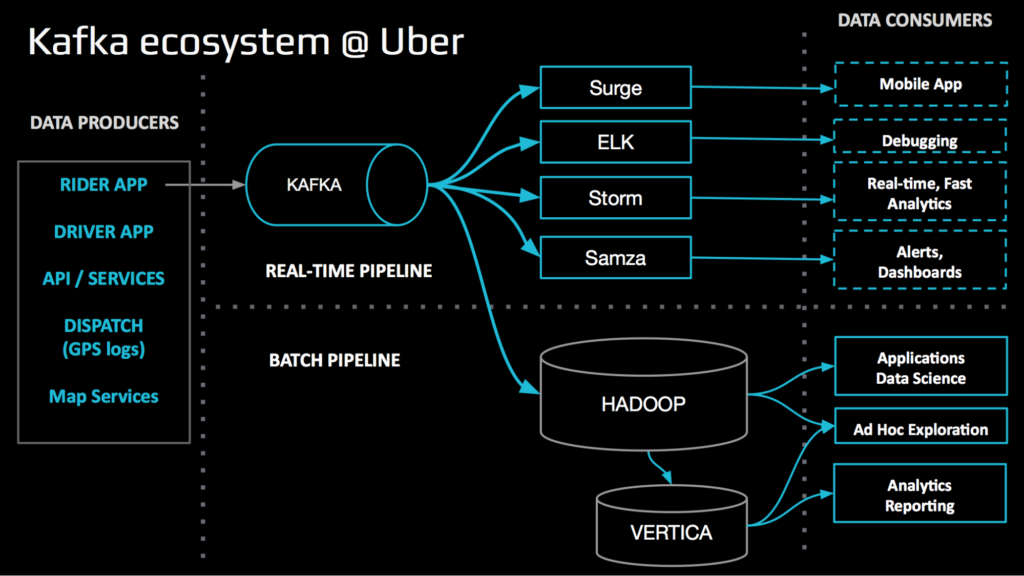
\includegraphics[scale=0.3]{kafka.png}
\caption{کافکا}
\label{fig:kafka}
\end{figure}


\section{تست در \lr{Uber}}
برای اطمینان از اینکه سرویس‌ها قادر به پاسخگویی به تقاضای محیط واقعی هستند، مهندسین در \lr{Uber}  دو نرم افزار \lr{uDestroy} و \lr{Hailstom} را برای تست میکروسرویس‌‌ها ایجاد کرده‌اند.\lr{Hailstorm} تست های ادغام را انجام می‌دهد و زمان اوج بار را نیز شبیه‌سازی می‌کند، در حالی که \lr{uDestroy} عمداً کارها را خراب می کند تا سیستم بتواند در کنترل خرابی های غیر منتظره بهتر عمل کند.

کارمندان \lr{Uber} قبل از اینکه برنامه به دست کاربران برسند، از نسخه بتا برنامه برای آزمایش مداوم تحولات جدید استفاده می کنند و در طی استفاده از نسخه بتا باگ ها را گزارش و ثبت می‌کنند.\cite{techstack}


\section{قابلیت اطمینان و مشاهده‌پذیری در \lr{Uber}}
شرکت \lr{Uber} برای نظارت از سامانه‌ی \lr{Nagios}\cite{Nagios} استفاده می‌کند،که به یک سیستم هشدار برای اعلان‌ها متصل است.در صورتی که کدی در بک‌اند منجر به شکست سیستم شود به مهندسان مربوطه اعلان ارسال می‌شود.

شرکت \lr{Uber} به منظور مانیتورینگ شرایط بخش‌های مختلف سازمان نرم‌افزار \lr{M3}\cite{m3} را گسترش داده است که که هر سخت افزار و کد توسط این نرم‌افزار تحت نظر قرار دارد.همچنین این شرکت از نرم افزار‌های تشخیص ناهنجاری نظیر \lr{Argos}\cite{argos} برای تشخص ناهنجاری‌ها بر اساس مدلی پیش‌بینی کننده مبین بر داده‌های گذشته استفاده می‌کند که در شکل \ref{fig:argos} نمایی از آن را مشاهده می‌شود.

\begin{figure}[h]
\centering
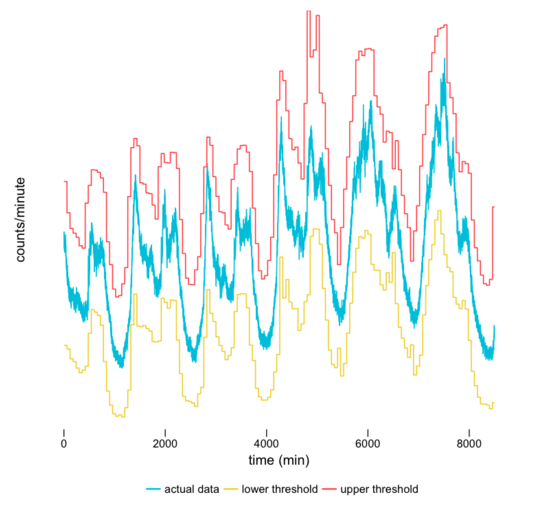
\includegraphics[scale=0.5]{argos.png}
\caption{\lr{Argos}}
\label{fig:argos}
\end{figure}








